% Cápitulo 3

\chapter{Uma arquitetura para a Rede Mocambos}
\label{Capitolo3}
\lhead{C\'apitulo 3. \emph{Uma arquitetura para Rede Mocambos}}

\section{Especificação dos requisitos}
A Rede Mocambos atualmente envolve cerca de 200 comunidades
localizadas em todo o território nacional brasileiro e algumas
comunidades na Africa e na Europa. A conectividade no Brasil é por
satélite, garantida pelo GESAC que disponibiliza para cada comunidade
uma \emph{Very Small Aperture Terminal} (VSAT) com banda de 512 kbit/s
em download e 128 kbit/s em upload. A topologia da rede é a estrela
então todos os nós comunicam por satélite concentrando o trafego num
\emph{hub} terrestre, onde a rede via satélite é interligada a
Internet. Cada comunidade tem uma sala com 10 computadores com acesso
publico, recém instalados (ou sendo instalados) pelo
Telecentros.BR\footnote{``O Programa Nacional de Apoio à Inclusão
  Digital nas Comunidades – Telecentros.BR é uma ação do Governo
  Federal de apoio à implantação de novos espaços públicos e
  comunitários de inclusão digital e o fortalecimento dos que já estão
  em funcionamento em todo o território. São disponibilizados
  equipamentos de informática e mobiliário necessários ao
  funcionamento dos telecentros, serviços de conexão em banda larga à
  internet, assim como a formação e bolsas de auxílio financeiro para
  monitores atuarem como agentes de inclusão digital. Esses monitores
  bolsistas participam de um curso de formação e atendem as
  comunidades dos telecentros.'', retirado de
  \url{http://www.inclusaodigital.gov.br/telecentros}.}, outro
programa do governo federal. A população de casa comunidade varia
desde as centenas as milhares de pessoas. A maioria das comunidade se
encontra em área rural, geralmente de difícil acesso e sem outros
meios de comunicação. Além dos espaços comunitários, normalmente
concentrados na zona central, a população é dividida em pequenos
núcleos familiares espalhados no território e as vezes muito distantes
um dos outros.

Vejamos agora alguns requisitos essenciais para essa arquitetura de
rede federada.

\subsection{Identidade de rede}
Os usuários das comunidades tem que ter identidade digitais com as
quais acessar e usar os serviços existentes. Além de acessar
localmente, é importante ter acesso a alguns serviços também fora da
própria comunidade. Por exemplo, no caso uma pessoa se encontra na
cidade, ela deve poder acessar, através da internet, aos serviços de
base, como o e-mail, o aos portais e serviços web da RM. É necessária
então uma identidade digital de rede univoca. 

\subsection{Autenticação descentralizada}
\label{sec:AutDec}
Um requisito essencial para cada comunidade é ter autonomia em
ausência de conexão internet, e a presença então de um sistema local
de autenticação e autorização. Além de garantir a continuidade do
serviço (em relação a problemas da conexão por satélite), é um
requisito importante para um bom desempenho de todos os serviços autenticados. 

\subsection{Sincronização}\label{Sincronizazzione}
A troca de informações entre as comunidades é o objetivo primário para
a RM. É então necessário um sistema para a sincronização seletiva dos
conteúdos de interesse geral. Para otimizar o uso da banda, as
operações de sincronização dos dados tem que influenciar o minimo
possível o uso quotidiano da internet, programando essas operações
durante a noite o de qualquer forma quando a conexão por satélite não
ta sendo usada. 

\subsection{Replicabilidade}
Cada comunidade se organiza autonomamente para a gestão da própria
infraestrutura tecnológica e as soluções adotadas tem então que ser
facilmente implementáveis e adaptáveis localmente. As ferramentas
precisam ser então soluções estáveis e possivelmente de uso comum,
também ao fim de encontrar mais facilmente assistência em loco. 

\subsection{Manutenção}
A manutenção do sistema tem que prever seja intervenções a distancia
seja locais. O sistema é baseado em tecnologias \emph{standard} e
abertas para garantir o acesso aos dados mesmo em caso de problemas.

\subsection{Desenvolvimento}
Cada comunidade tem características e necessidades próprias que levam
a serviços diferenciados. A arquitetura geral da RM tem que ser uma
base estável em cima da qual poder desenvolver sem demais restrições.
As tecnologias e as linguagens adotadas tem que facilitar a interação,
a formação e o reuso dos conhecimentos. 

\section{Ferramentas e praticas para o desenvolvimento}
Pela natureza da RM, e em particular pela necessidade de autonomia
tecnológica, a formação é fundamental então é importante o uso de
ferramentas que facilitem a documentação e o desenvolvimento
colaborativo. A RM já utiliza a anos um wiki\footnote{``Un Wiki é uma
  pagina (ou uma coleção de hipertextos) que é atualizada pelos seus
  usuários e cujos conteúdos são desenvolvidos colaborativamente por
  todos que tenham acesso. A alteração dos conteúdos é aberta, no
  sentido que o texto pode ser modificado por todos os usuários (as
  vezes mesmo se anônimos) contribuindo non somente adicionando, como
  acontece normalmente nos fóruns, mas também mudando e excluindo o
  que outros escreveram. Cada mudança fica gravada em uma cronologia
  que permite, quando necessário, voltar a versão antecedente; o
  objetivo é compartilhar, trocar, armazenar e otimizar os
  conhecimentos de maneira colaborativa. O termo wiki indica também o
  software utilizado para criar o site web num servidor.'', traduzido
  de \url{http://it.wikipedia.org/wiki/Wiki}.}, disponível no endereço
\url{http://wiki.mocambos.net}, onde se encontra parte da documentação
sobre o sistema e o código desenvolvido para este trabalho. Para o
versionamento do código foi usado o sistema descentralizado GIT (ver
\ref{sec:GIT}) e a plataforma
GITHUB\footnote{\href{http://github.com}{GITHUB} è uma rede social
  baseada no sistema GIT \ref{sec:GIT}.}. O código do protótipo é
disponível no endereço \url{https://github.com/RedeMocambos}.

\subsection{Sistema operacional}
A escolha de um sistema operacional comum facilita a documentação, a
automação e a assistência a distancia. Muitas comunidades já usam
distribuições GNU/Linux baseadas no Debian\footnote{``O Projeto Debian
  é uma associação de indivíduos que têm como causa comum criar um
  sistema operacional livre. O sistema operacional que criamos é
  chamado Debian GNU/Linux, ou simplesmente Debian.'', retirado de
  \url{http://www.debian.org}}. Para o protótipo foram escolhidas as
ultimas versões estáveis do Debian, a 6.0, e de
Ubuntu\footnote{``Ubuntu é um sistema operacional GNU/Linux criado em
  2004, baseado no Debian, focado no usuário e na facilidade de
  uso. Ubuntu é orientado para uso em desktop e dando muita atenção ao
  suporte do hardware. A cada seis meses é lançada uma nova
  versão. Financiado pela empresa Canonical Ltd (com registro na Ilha
  de Man), este sistema é compartilhado como Software Livre sob
  licença GNU GPL.'', traduzido de
  \url{http://it.wikipedia.org/wiki/Ubuntu}.}, a 11.10.

\subsection{Linguagens de programação}
Para o sistema desenvolvido foi escolhida a linguagem de programação
Python, uma linguagem muito flexível e provavelmente o mais versátil
para conectar componentes heterogêneas. Várias comunidades já usam
Software Livres como: \emph{GIMP}\footnote{\emph{GNU Image
    Manipulation Program (GIMP)} é um programa para edição, montagem e
  criação de imagens. Disponível em \url{http://www.gimp.org/}.},
\emph{Blender}\footnote{\emph{Blender} é um programa para a criação de
  gráfica e ambientes tridimensionais. Disponível em
  \url{http://www.blender.org/}.},
\emph{Inkscape}\footnote{\emph{Inkscape} é um programa de gráfica
  vectorial conforme ao formado SVG. Disponível em
  \url{http://inkscape.org}.} que também fazem uso de \emph{scripting}
Python para criação de filtros e para outras funcionalidades
avançadas.

\subsection{Virtualização}
O protótipo foi desenvolvido e testado em um ambiente virtualizado,
para garantir maior controle e verificar a exatidão dos procedimentos
em todos seus passos. Os \emph{script} para automatizar as
instalações, e os procedimentos passo a passo na documentação, foram
feitos a partir da configuração de base do sistema. Foram criadas
maquinas virtuais, com a ajuda do software livre
\emph{VirtualBox}\footnote{\emph{VirtualBox} é um virtualizador
  completo para arquiteturas x86 para uso em servidores, desktop e
  sistemas embutidos. Disponível em
  \url{http://www.virtualbox.org/}.}, simulando os servidores
comunitários/locais e o servidor central.

\section{Arquitetura base}

\subsection{Gestão das identidades de rede}
Analisando a especificação dos requisitos e algumas das tecnologias
existentes que vimos no capítulo precedente, foi escolhido o uso de
LDAP para gerenciar as credenciais dos usuários da RM. O protótipo
proposto prevê um servidor central em conectividade internet garantida
e servidores locais em replicação. É possível uma configuração onde
todos os servidores da rede sejam \emph{master} (modalidade
\emph{N-Way-Multimaster}). Esta configuração, se por um lado permite a
atualização em escritura das bases dos usuários em cada servidor, por
outro lado pode gerar mais facilmente situações de inconsistência dos
dados e problemas de sincronização entre os servidores LDAP. Por esta
razão para o protótipo realizado se escolheu relaxar o requisito
\ref{sec:AutDec}, assumindo um síngulo servidor \emph{master} para
toda a rede onde efetuar as operações de escritura (criação,
eliminação, e atualização dos usuários) e servidores locais
habilitados somente para operações em leitura. Cada comunidade então
teria a disposição um servidor LDAP replicado para autenticação e
autorização. Contudo, na falta da conexão esterna, os serviços locais
permanecem ativos para os usuários habilitados até a ultima
sincronização. 

\subsection{Mocambos\_LDAP}\label{MocambosLDAP}
\framebox[\textwidth]{\footnotesize O código esta disponível em
\url{https://github.com/RedeMocambos/Mocambos_LDAP}}

Para facilitar a implementação dos servidores LDAP por parte dos
administradores locais, foi desenvolvido um \emph{script} de
instalação, que pode se tornar útil também para um administrador
remoto. O \emph{script} instala os pacotes necessários e prepara o
servidor LDAP \emph{slapd} em configuração \emph{master} ou
replica. Também cria um DIT pré-configurado para a RM com uma simples
estrutura (ver figura \ref{fig:DIT_ReteMocambos}).

\begin{figure}[htbp]
  \centering
  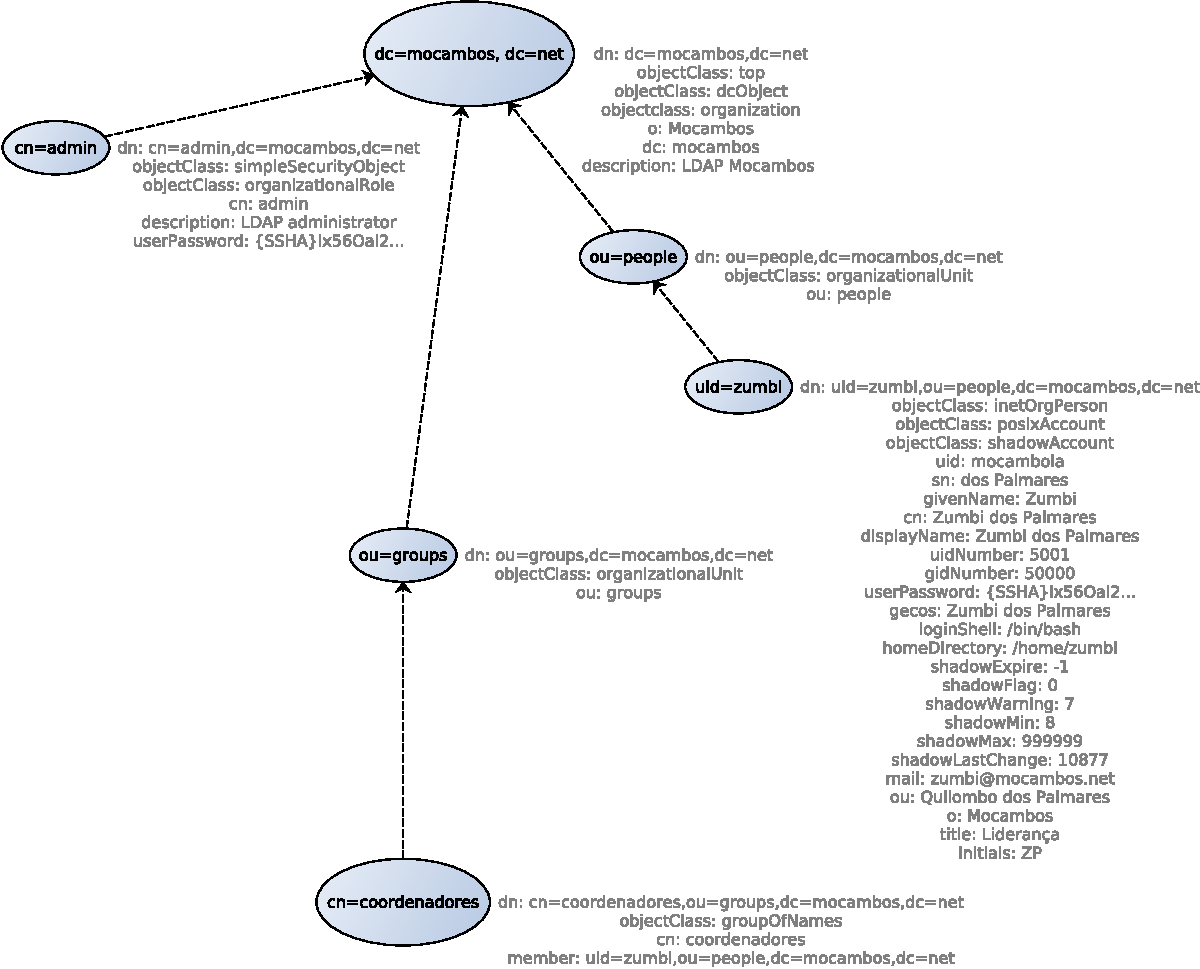
\includegraphics[width=\textwidth]{./Figure/DIT_ReteMocambos-crop.pdf}
  \rule{35em}{0.5pt}
  \caption[DIT base do servidor LDAP da RM]{DIT base do servidor LDAP da RM.}
  \label{fig:DIT_ReteMocambos}
\end{figure}




